\documentclass[tikz,border=4pt]{standalone}
\usepackage{pgfplots}\usepgfplotslibrary{groupplots}
\pgfplotsset{compat=1.18}
\definecolor{corba}{HTML}{365FB3}\definecolor{punt}{HTML}{B91C1C}
\begin{document}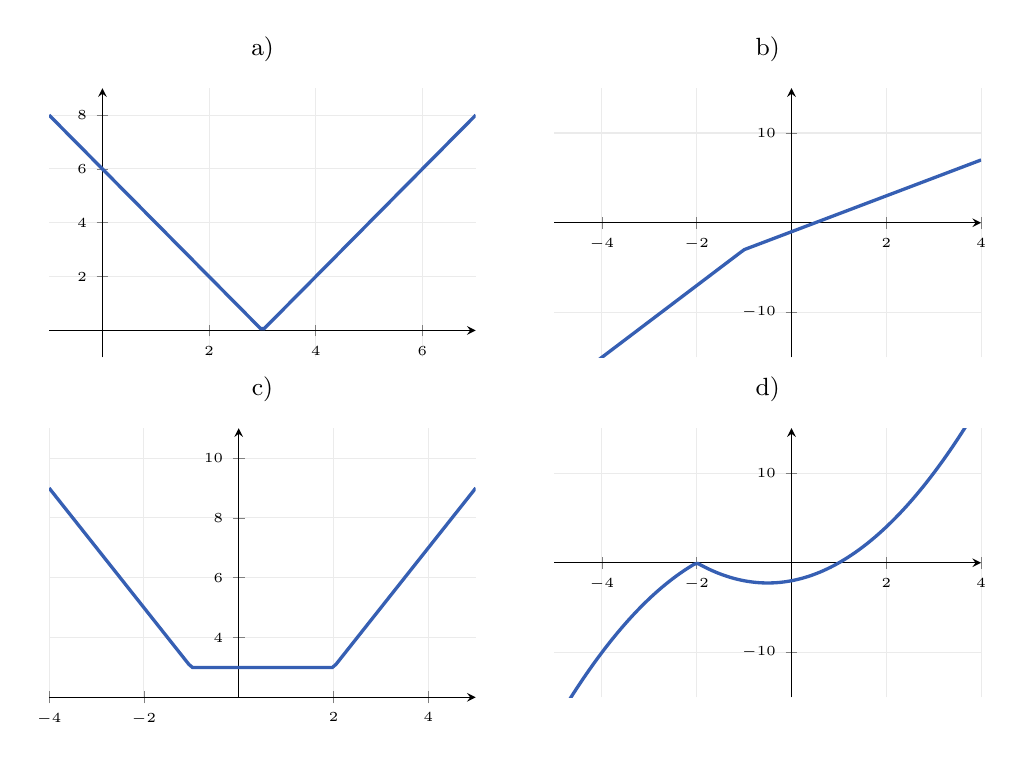
\begin{tikzpicture}
\begin{groupplot}[group style={group size=2 by 2,horizontal sep=1cm,vertical sep=0.9cm},width=7cm,height=5cm,
 axis lines=middle,grid=major,grid style={black!8},tick label style={font=\tiny},title style={font=\small},samples=120]
\nextgroupplot[title={a)},xmin=-1,xmax=7,ymin=-1,ymax=9]\addplot[corba,very thick,domain=-1:7]{abs(2*x-6)};
\nextgroupplot[title={b)},xmin=-5,xmax=4,ymin=-15,ymax=15]\addplot[corba,very thick,domain=-5:4]{3*x-abs(x+1)};
\nextgroupplot[title={c)},xmin=-4,xmax=5,ymin=2,ymax=11]\addplot[corba,very thick,domain=-4:5]{abs(x+1)+abs(x-2)};
\nextgroupplot[title={d)},xmin=-5,xmax=4,ymin=-15,ymax=15]\addplot[corba,very thick,domain=-5:4]{(x-1)*abs(x+2)};
\end{groupplot}\end{tikzpicture}\end{document}
